% Adjust these for the path of the theme and its graphics, relative to this file
%\usepackage{beamerthemeFalmouthGamesAcademy}
\usepackage{../../beamerthemeFalmouthGamesAcademy}
\usepackage{multimedia}
\graphicspath{ {../../} }

% Default language for code listings
\lstset{language=C++,
        morekeywords={each,in,nullptr}
}

% For strikethrough effect
\usepackage[normalem]{ulem}
\usepackage{wasysym}

\usepackage{pdfpages}

% http://www.texample.net/tikz/examples/state-machine/
\usetikzlibrary{arrows,automata}

\newcommand{\modulecode}{COMP260}\newcommand{\moduletitle}{Distributed Systems}\newcommand{\sessionnumber}{5}

\begin{document}
\title{\sessionnumber: The graphics pipeline}
\subtitle{\modulecode: \moduletitle}

\frame{\titlepage} 

\begin{frame}
	\frametitle{Learning outcomes}
	By the end of today's session, you will be able to:
	\begin{itemize}
		\item \textbf{Recall} the key stages of the graphics pipeline
		\item \textbf{Explain} the differences between a CPU and a GPU
		\item \textbf{Write} basic programs using SDL and OpenGL
	\end{itemize}
\end{frame}

\part{Course introduction}
\frame{\partpage}

\begin{frame}{From the module guide}
This module will introduce you to the techniques of 3D graphics rendering and physics simulation used in modern computer games. Using the OpenGL library, you will develop an understanding of the 3D graphics pipeline, and how to program the GPU to produce advanced graphical effects.
\end{frame}

\begin{frame}{Topic schedule}
	\begin{center}
		On LearningSpace...
	\end{center}
\end{frame}

\begin{frame}{Assignment 1: Portfolio task}
	\begin{center}
		First worksheet is due in week 4.
	\end{center}
\end{frame}

\begin{frame}{Assignment 2: Research journal}
	\begin{center}
		First component due in week 3.
		\pause Don't forget to update the wiki!
	\end{center}
\end{frame}


% http://tex.stackexchange.com/questions/30720/footnote-without-a-marker
\newcommand\blfootnote[1]{%
  \begingroup
  \renewcommand\thefootnote{}\footnote{#1}%
  \addtocounter{footnote}{-1}%
  \endgroup
}

\part{Graphics and simulation hardware}
\frame{\partpage}

\begin{frame}{CPUs vs GPUs}
	\begin{itemize}
		\item (CPU = central processing unit; GPU = graphics processing unit)
		\pause \item GPUs are \textbf{highly parallelised}
			\begin{itemize}
				\pause \item Intel i7 6900K: \textbf{8} cores
				\pause \item Nvidia GTX 1080: \textbf{2560} shader processors
			\end{itemize}
		\pause \item GPUs are \textbf{highly specialised}
			\begin{itemize}
				\pause \item Optimised for floating-point calculations rather than logic
				\pause \item Optimised for performing the same calculation on several thousand vertices or pixels at once
			\end{itemize}
	\end{itemize}
\end{frame}

\begin{frame}{General purpose GPU (GPGPU)}
	\begin{itemize}
		\item Early GPUs used a \textbf{fixed pipeline} -- could only be used for rendering 3D graphics
		\pause \item Modern GPUs use a \textbf{programmable pipeline} -- can be programmed for other tasks
		\pause \item Physics simulation (e.g.\ PhysX)
		\pause \item Scientific computing (e.g.\ CUDA)
		\pause \item Deep learning
	\end{itemize}
\end{frame}

\begin{frame}{Graphics APIs}
	\begin{itemize}
		\item Graphics APIs \textbf{abstract} away the differences between different manufacturers' GPUs
		\pause\item There are several APIs in use today:
		\begin{itemize}
			\pause\item \textbf{OpenGL}: Open standard, very mature, very widely supported
			\pause\item \textbf{Vulkan}: Open standard, less mature, lots of control on rendering, lots of work to get a basic sample working
			\pause\item \textbf{Direct3D}: Microsoft only
			\pause\item \textbf{Metal}: Apple only
			\pause\item Sony and Nintendo consoles have their own APIs; Microsoft consoles use Direct3D
		\end{itemize}
	\end{itemize}
\end{frame}

\begin{frame}{Game Engines \& Graphic APIs}
\begin{itemize}
	\item Game Engines tend to support multiple Graphics API
	\pause \item They using have an abstract rendering layer which has concrete implementations of D3D, OpenGL, Vulkan, Metal, Console APIs etc
	\pause \item This allows the Engine to support multiple platforms
	\pause \item In addition, this makes it easier to upgrade the engine to support new versions of APIs or newly released APIs
\end{itemize}
\end{frame}


%Add in the other shader stages(Tesselation and Geometry)
\part{The 3D graphics pipeline}
\frame{\partpage}

\begin{frame}{The 3D graphics pipeline}
	\begin{center}
		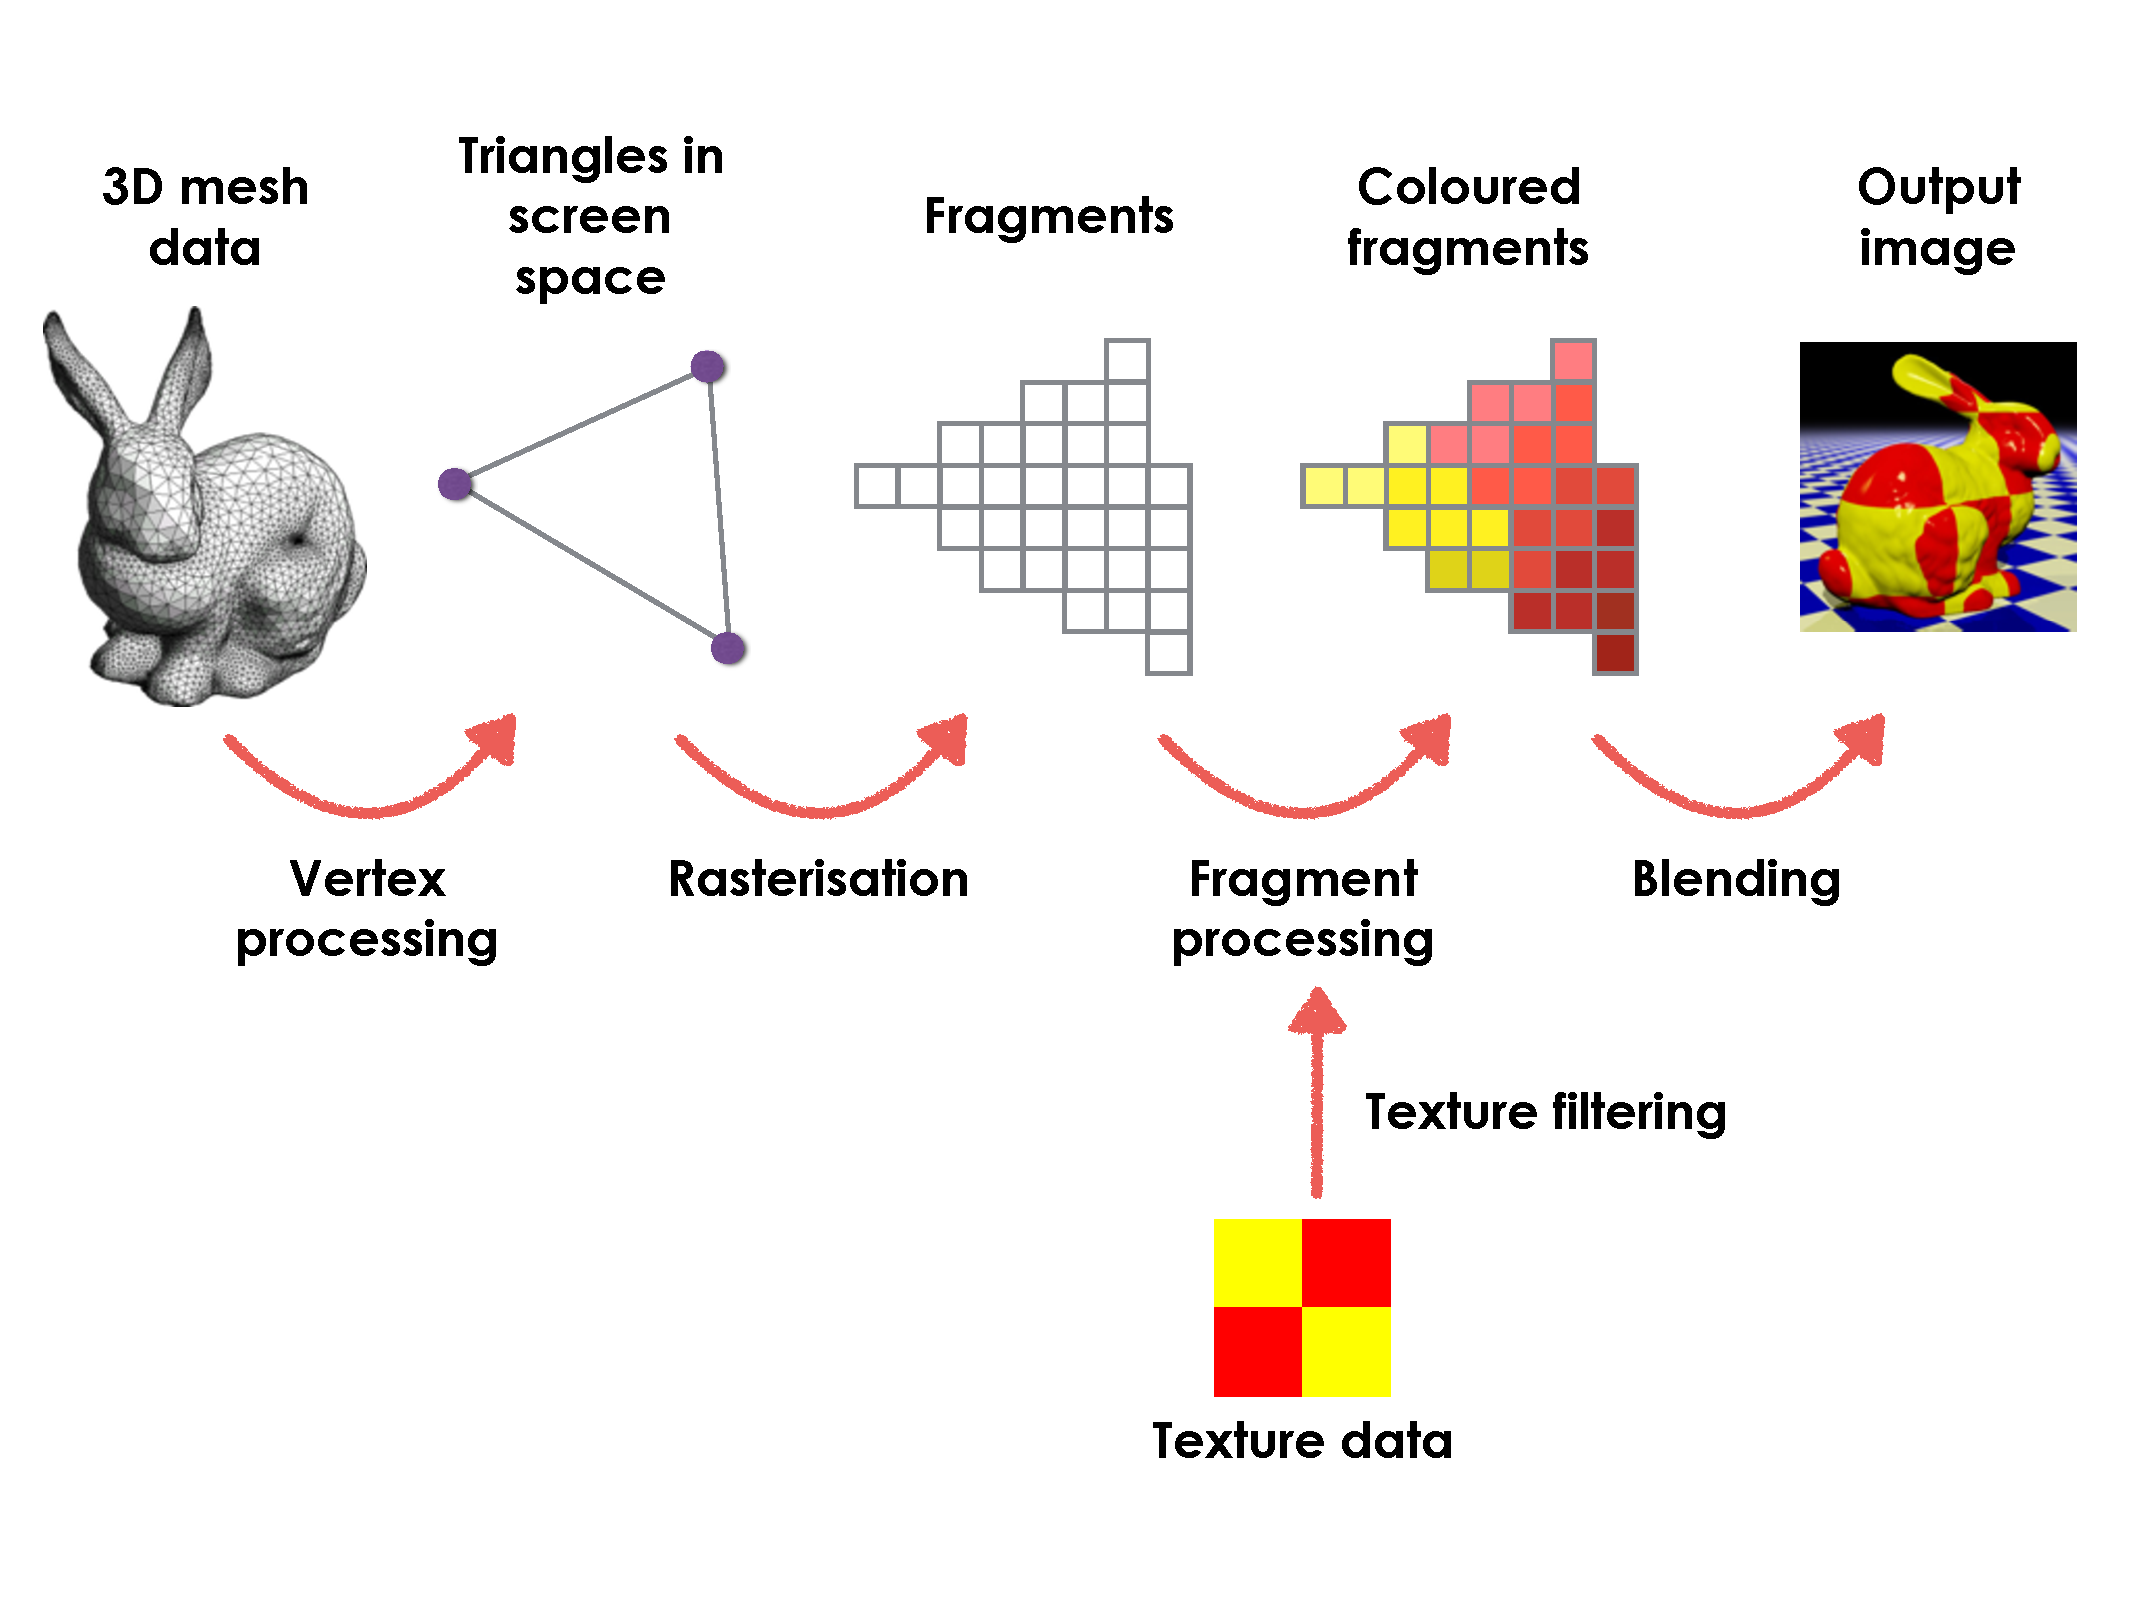
\includegraphics[height=0.7\textheight]{pipeline}
	\end{center}
\end{frame}

\begin{frame}{Vertex processing}
	\begin{columns}
		\begin{column}{0.3\textwidth}
			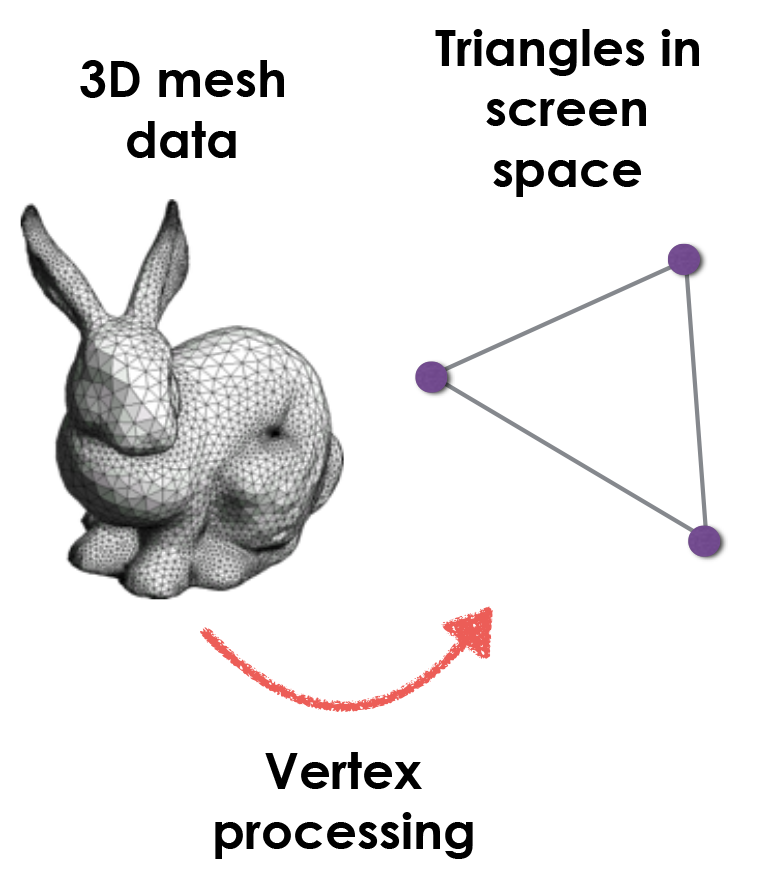
\includegraphics[width=\textwidth]{pipeline_1}
		\end{column}
		\begin{column}{0.65\textwidth}
			\begin{itemize}
				\pause\item Geometry is provided to the GPU as a \textbf{mesh} of \textbf{triangles}
				\pause\item Each triangle has three \textbf{vertices} specified in 3D space $(x,y,z)$
				\pause\item Vertex processor \textbf{transforms} (rotates, moves, scales) vertices
					and \textbf{projects} them into 2D screen space $(x,y)$
				\pause\item May also apply particle simulations, skeletal animations or deformations, etc.
			\end{itemize}
		\end{column}
	\end{columns}
\end{frame}

\begin{frame}{Rasterisation}
	\begin{columns}
		\begin{column}{0.3\textwidth}
			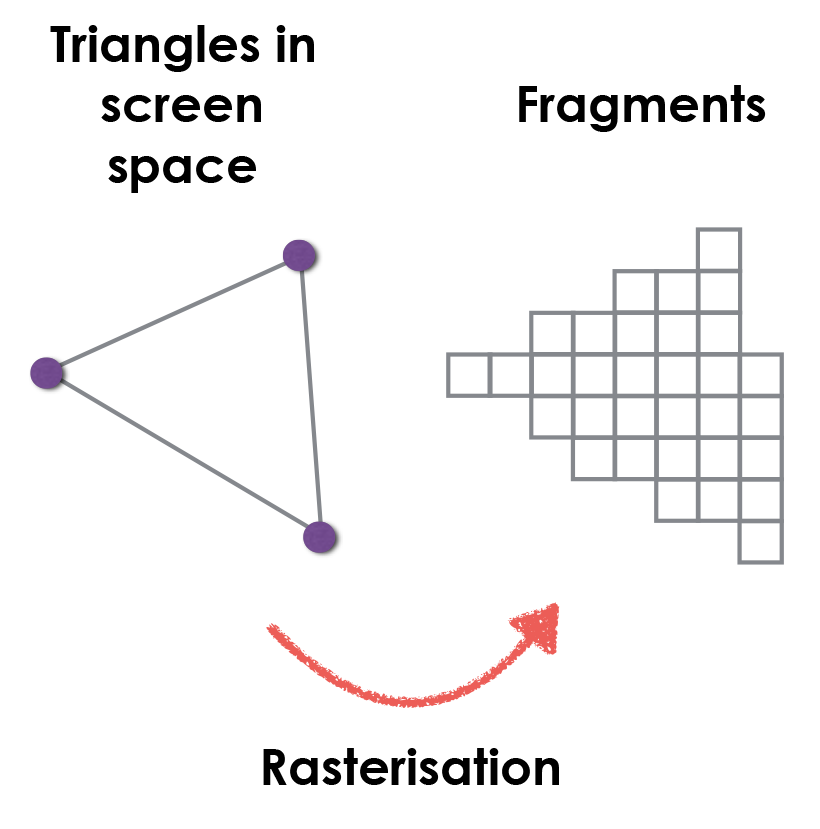
\includegraphics[width=\textwidth]{pipeline_2}
		\end{column}
		\begin{column}{0.65\textwidth}
			\begin{itemize}
				\pause\item Determine \textbf{which fragments} are covered by the triangle
				\pause\item In practical terms, ``fragment'' = ``pixel''
				\pause\item Vertex processor can associate \textbf{data} with each vertex;
					this is \textbf{interpolated} across the fragments
			\end{itemize}
		\end{column}
	\end{columns}
\end{frame}

\begin{frame}{Fragment processing}
	\begin{columns}
		\begin{column}{0.3\textwidth}
			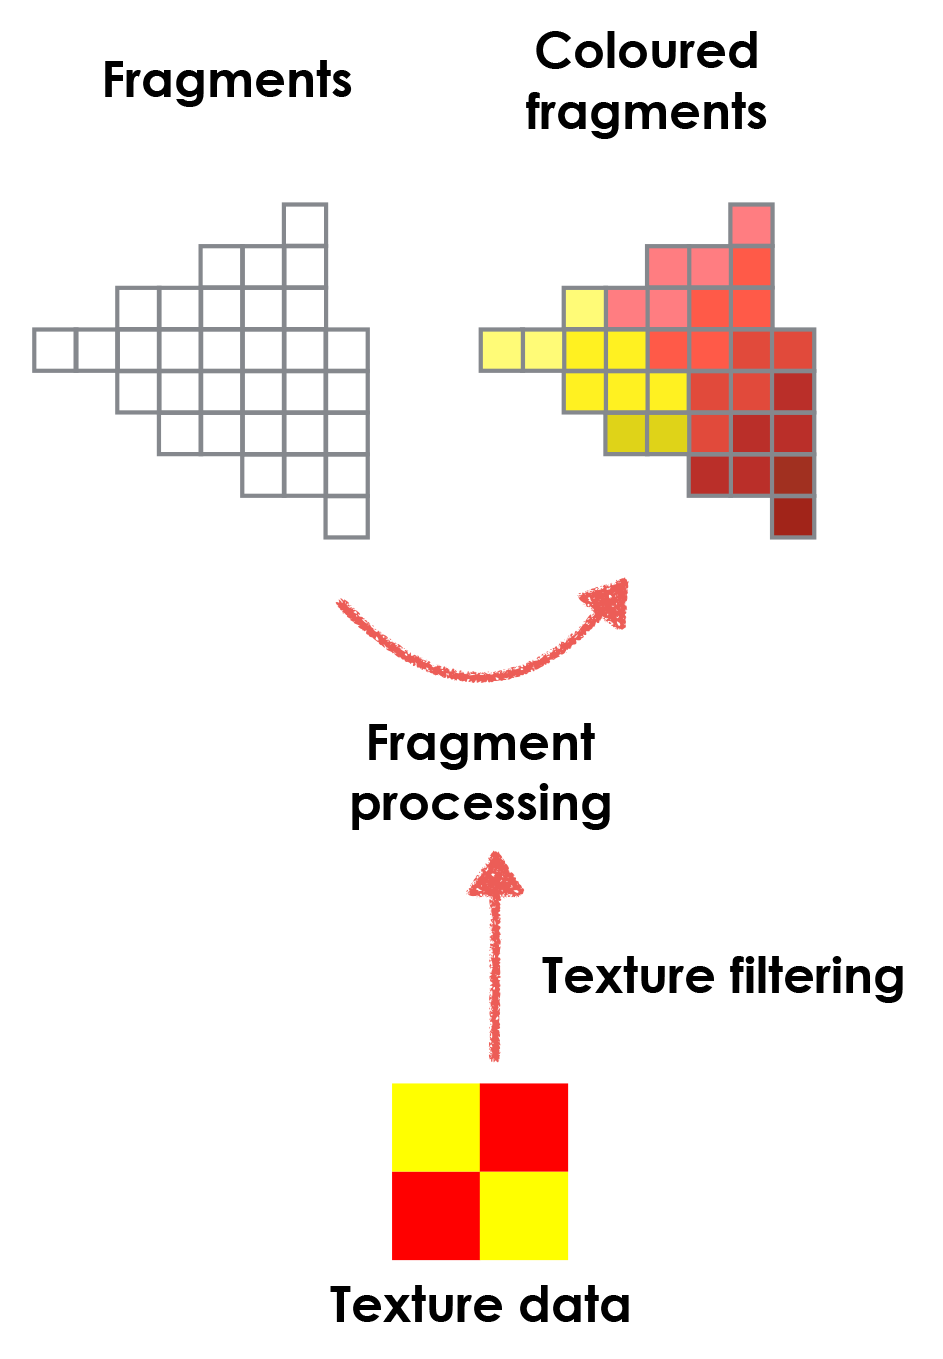
\includegraphics[width=\textwidth]{pipeline_3}
		\end{column}
		\begin{column}{0.65\textwidth}
			\begin{itemize}
				\pause\item Determine the \textbf{colour} of each fragment covered by the triangle
				\pause\item \textbf{Textures} are 2D images that can be \textbf{wrapped} onto a 3D object
				\pause\item Colour is calculated based on \textbf{texture}, \textbf{lighting} and other
					properties of the surface being rendered (e.g.\ shininess, roughness)
			\end{itemize}
		\end{column}
	\end{columns}
\end{frame}

\begin{frame}{Blending}
	\begin{columns}
		\begin{column}{0.3\textwidth}
			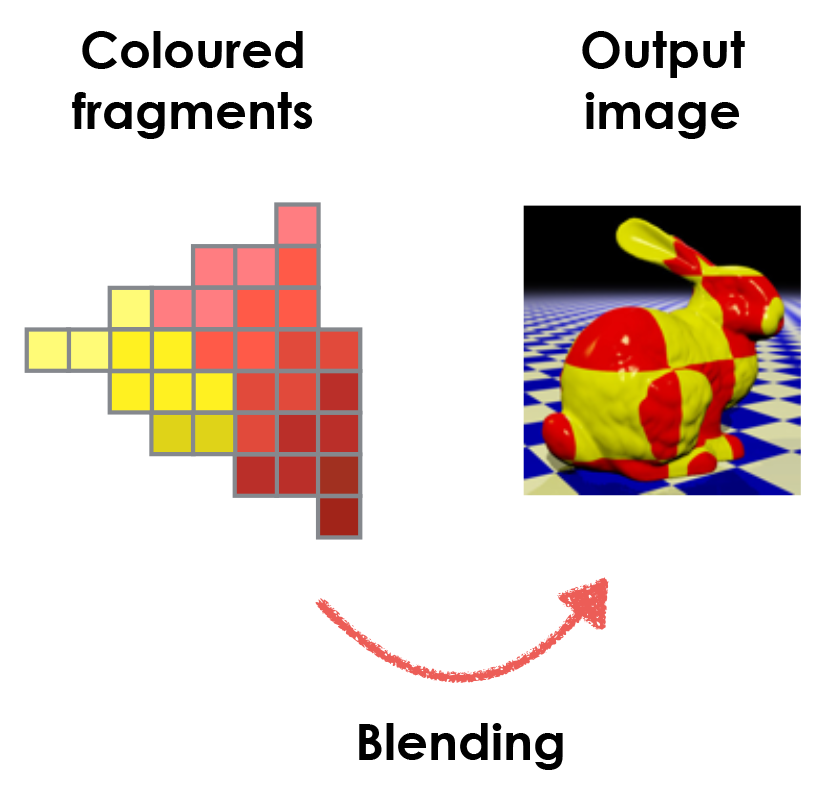
\includegraphics[width=\textwidth]{pipeline_4}
		\end{column}
		\begin{column}{0.65\textwidth}
			\begin{itemize}
				\pause\item Combine these fragments with the existing content of the image buffer
				\pause\item \textbf{Depth testing}: if the new fragment is ``in front'' of the old one, replace it;
					if it is ``behind'', discard it
				\pause\item \textbf{Alpha blending}: combine the old and new colours for a semi-transparent appearance
			\end{itemize}
		\end{column}
	\end{columns}
\end{frame}

\begin{frame}{Shaders}
	\begin{itemize}
		\pause\item The vertex processor and fragment processor are \textbf{programmable}
		\pause\item Programs for these units are called \textbf{shaders}
		\pause\item \textbf{Vertex shader}: responsible for geometric transformations, deformations, and projection
		\pause\item \textbf{Fragment shader}: responsible for the visual appearance of the surface
		\pause\item Vertex shader and fragment shader are separate programs,
			but the vertex shader can pass arbitrary values through to the fragment shader
	\end{itemize}
\end{frame}



\part{Your first OpenGL program}
\frame{\partpage}

\begin{frame}{SDL and OpenGL}
	\begin{itemize}
		\pause\item OpenGL only handles rendering of graphics
		\pause\item We need something else to handle windows, events, audio etc
		\pause\item We will use \textbf{SDL} (which you have used before, via PyGame)
	\end{itemize}
\end{frame}

\begin{frame}{Live coding}
	\begin{center}
		\url{https://github.com/Falmouth-Games-Academy/bsc-live-coding}
	\end{center}
\end{frame}

\begin{frame}{Live coding - basics}
	\begin{center}
		\url{http://headerphile.com/sdl2/opengl-part-1-sdl-opengl-awesome/}
	\end{center}
\end{frame}

\begin{frame}{Our first triangle}
	\begin{center}
		\url{http://www.opengl-tutorial.org/beginners-tutorials/tutorial-2-the-first-triangle/}
	\end{center}
\end{frame}



\begin{frame}
	\frametitle{Debrief}
	It's the end of today's session. You are now able to:
	\begin{itemize}
		\item \textbf{Recall} the key stages of the graphics pipeline
		\item \textbf{Explain} the differences between a CPU and a GPU
		\item \textbf{Write} basic programs using SDL and OpenGL
	\end{itemize}
	Don't forget! Portfolio task proposals due \textbf{this time next week!}
\end{frame}

\end{document}
